\documentclass[a4paper,11pt]{article}

\usepackage[utf8]{inputenc}
\usepackage[T1]{fontenc}
\usepackage{lmodern}
\usepackage{amsmath,amssymb}
\usepackage{graphicx}
\usepackage{booktabs}
\usepackage{siunitx}
\usepackage{hyperref}
\usepackage{geometry}
\usepackage{titlesec}
\usepackage{setspace}
\usepackage{enumitem}
\setlength{\parindent}{1cm}
\setlength{\parskip}{0.5em}

\geometry{margin=3cm}
\onehalfspacing

% Configure list spacing
\setlist[itemize]{itemsep=0.5em, parsep=0.3em, topsep=0.5em}
\setlist[enumerate]{itemsep=0.5em, parsep=0.3em, topsep=0.5em}

\sisetup{
  round-mode=places,
  round-precision=6,
  scientific-notation=false
}

\title{\textbf{Efficient Minimization of Continuous Mathematical Functions using Real-Coded Genetic Algorithms}}
\author{Negura Teodor Alexandru \\ \\ \textbf{"University A.I. Cuza"}}
\date{}

\begin{document}
\titleformat{\section}{\centering\normalfont\huge\bfseries}{}{0em}{}[\vspace{0.5em}]
\titleformat{\subsection}{\centering\normalfont\Large\bfseries}{}{0em}{}[\vspace{0.3em}]
\titleformat{\subsubsection}{\centering\normalfont\large\bfseries}{}{0em}{}[\vspace{0.2em}]
\titlespacing*{\section}{0pt}{2em}{1.5em}
\titlespacing*{\subsection}{0pt}{1.5em}{1em}
\titlespacing*{\subsubsection}{0pt}{1em}{0.5em}
\maketitle
\thispagestyle{empty}

\begin{abstract}
This report studies the minimization of four standard continuous benchmark functions --
De~Jong~1, Rastrigin, Schwefel and Michalewicz -- using a real-coded Genetic Algorithm (GA).
The work corresponds to The Second Assignment, and extends the local-search methods from
The First Assignment: hill climbing (First / Best / Worst Improvement) and Simulated Annealing (SA).

The objective is twofold: 
(i) to design and implement a robust real-coded GA capable of
reaching high precision (at least five correct decimal digits) in dimensions up to 30, and
(ii) to compare empirically the performance of the GA against the H1 baselines, in terms
of solution quality and robustness. For each configuration (function, dimension, algorithm),
30 independent runs are performed and the statistics of the final best fitness are reported
(best, mean, standard deviation, worst, and mean error with respect to the known optimum).

The experiments show that, while hill climbing and SA can perform reasonably well on
unimodal functions in low dimension, they quickly deteriorate in higher dimensional and
highly multimodal landscapes. In contrast, the real-coded GA systematically achieves
near-optimal solutions on all four benchmark problems in 30 dimensions, often reaching
machine precision on De~Jong~1 and Rastrigin, and significantly improving over SA on
Schwefel and Michalewicz.
\end{abstract}

\section{Introduction}

Continuous optimization problems appear in almost every scientific and engineering domain:
parameter tuning of physical models, machine learning, signal processing, control, and many
others. In many cases, the objective function is non-convex, noisy or non-differentiable,
and gradient-based methods are either inapplicable or become trapped in poor local optima.

Metaheuristics such as hill climbing, Simulated Annealing and Genetic Algorithms provide
a flexible framework for such black-box optimization problems. The First Assignment focused
on local-search methods (several variants of hill climbing and SA) applied to four standard
benchmark functions: De~Jong~1, Rastrigin, Schwefel and Michalewicz, in dimensions
$5$, $10$, $30$ and $100$. While The First Assignment demonstrated that local search can significantly improve
over random search, it also highlighted important limitations:
\begin{itemize}
  \item hill climbing variants are strongly affected by local minima and plateaus;
  \item Simulated Annealing is more robust, but still degrades rapidly as dimensionality
        and multimodality increase;
  \item obtaining high precision (five or more correct decimal digits) in 30 dimensions
        is extremely difficult with purely local moves.
\end{itemize}

The Second Assignment addresses these limitations by moving from single-solution local search
to a population-based evolutionary algorithm: a real-coded Genetic Algorithm.
The main goals of this report are:
\begin{enumerate}
  \item to describe the design choices of the GA (representation, variation operators,
        selection, elitism, parameter settings);
  \item to present a statistically sound experimental protocol (number of dimensions,
        repetitions, statistics) for comparing the GA with the The First Assignment methods;
  \item to analyse quantitatively how much the GA improves over hill climbing and SA
        on each benchmark function and dimensionality.
\end{enumerate}

\section{Methods}
\label{sec:methods}

\subsection{Benchmark functions and problem formulation}

We consider four standard continuous benchmark functions used in the course:
\begin{itemize}
  \item \textbf{De~Jong~1 (Sphere)}:
    \[
      f_{\mathrm{DJ1}}(x) = \sum_{i=1}^{d} x_i^2,
    \]
    with $x_i \in [-5.12, 5.12]$ and global minimum $f^\star = 0$ at $x^\star = 0$.
    This is a smooth, strictly convex and unimodal function.

  \item \textbf{Rastrigin}:
    \[
      f_{\mathrm{Ras}}(x) = 10 d + \sum_{i=1}^{d}
      \left(x_i^2 - 10 \cos (2\pi x_i)\right), \quad x_i \in [-5.12, 5.12],
    \]
    with global minimum $f^\star = 0$ at $x^\star = 0$. The function is highly
    multimodal, with a large number of regularly spaced local minima.

  \item \textbf{Schwefel}: we use the classical Schwefel function as defined in the
    course, with domain $x_i \in [-500,500]$. The function is deceptive: the
    global optimum is far from the origin, while many deep local minima are closer.

  \item \textbf{Michalewicz}:
    \[
      f_{\mathrm{Mich}}(x) =
      -\sum_{i=1}^{d} \sin(x_i)\left[\sin\!\left(\frac{i x_i^2}{\pi}\right)\right]^{2m},
    \]
    with $m=10$ and domain $x_i \in [0,\pi]$. The function has very sharp and narrow
    valleys and the global optimum is difficult to reach in high dimension.
\end{itemize}

In all cases, the task is to solve the minimization problem
\[
  \min_{x \in \mathcal{D} \subset \mathbb{R}^d} f(x)
\]
for dimensionalities $d \in \{5,10,30\}$ in The Second Assignment, and to compare with the corresponding
results from The First Assignment (which also included $d=100$).

\subsection{Local-search baselines from The First Assignment}

The First Assignment implemented four local-search strategies:
\begin{itemize}
  \item \emph{First Improvement hill climbing}: starting from a random point, repeatedly
    evaluates neighbours and moves to the first improving neighbour.
  \item \emph{Best Improvement hill climbing}: evaluates all neighbours and always moves
    to the best one.
  \item \emph{Worst Improvement hill climbing}: moves to the worst improving neighbour
    (more exploratory, but still greedy).
  \item \emph{Simulated Annealing (SA)}: a probabilistic local-search algorithm that
    accepts worsening moves with a probability depending on a temperature schedule.
\end{itemize}

In The First Assignment, the search was constrained by a maximum number of function evaluations
(e.g., around $2\,000\,000$ for $d=5$, $4\,000\,000$ for $d=10$ , $12\,000\,000$
for $d=30$) and $40\,000\,000$ for $d=100$), , and for each configuration (function, dimension, strategy) 50 independent
runs were performed. The final The First Assignment statistics (best, mean, standard deviation,
worst) are used here as the baseline to which the GA will be compared.%
\footnote{For brevity, we will focus on Simulated Annealing, which consistently
dominated the hill-climbing variants in The First Assignment.}

\subsection{Real-coded Genetic Algorithm (The Second Assignment)}

The Genetic Algorithm used in The Second Assignment is real-coded and population-based. It follows the
classical evolutionary loop:
\[
  \text{Initialize} \rightarrow \text{Evaluate} \rightarrow
  \text{Select} \rightarrow \text{Crossover} \rightarrow
  \text{Mutate} \rightarrow \text{Replace},
\]
with several specific design choices suited for continuous optimization.%
\footnote{The high-level design and motivation follow standard real-coded GA
literature and were guided by the course notes.}

\subsubsection{Representation and initialization}

Each individual encodes a candidate solution $x \in \mathbb{R}^d$ as a vector of
doubles:
\[
  x = (x_1, x_2, \dots, x_d) \in \mathbb{R}^d.
\]
This real-coded representation avoids the precision and Hamming-cliff issues
associated with binary encodings.

The initial population is generated by sampling each coordinate independently
from a uniform distribution over the domain of the corresponding function,
e.g.\ $x_i \sim \mathcal{U}[-5.12,5.12]$ for De~Jong~1 and Rastrigin.
This ensures that the initial population covers the whole search space and
does not introduce a bias towards any particular region.

\subsubsection{Fitness evaluation}

All four benchmark functions are minimization problems. The GA uses the raw
function value as fitness and implements selection and elitism in terms of
``lower is better''. No additional scaling or normalization is required, which
also simplifies comparison across algorithms.

\subsubsection{Selection: tournament selection}

Parent selection uses $k$-tournament selection with $k=3$:
\begin{enumerate}
  \item sample $k$ individuals uniformly at random from the population;
  \item choose the individual with the lowest fitness as the parent.
\end{enumerate}
Tournament selection is robust and independent of absolute fitness values,
making it suitable for functions with negative optima (e.g.\ Michalewicz,
Schwefel). By tuning $k$, the selection pressure can be controlled; in our
experiments $k=3$ offered a good balance between exploration and exploitation.

\subsubsection{Crossover: Simulated Binary Crossover (SBX)}

For recombination we use Simulated Binary Crossover (SBX), a standard operator
for real-coded GAs:
\begin{itemize}
  \item for each pair of parents $(x^{(1)}, x^{(2)})$ and each gene $i$, SBX
        generates two children $y^{(1)}_i$ and $y^{(2)}_i$ by sampling around
        the parents according to a distribution controlled by a parameter
        $\eta_c$ (the \emph{distribution index});
  \item when parents are close in a coordinate, children are also close, which
        favours exploitation; when parents are far apart, SBX explores the
        space between them.
\end{itemize}

We used a crossover probability $p_c = 0.9$ and a distribution index
$\eta_c = 15$. A high crossover rate, combined with tournament selection
and elitism, allows good building blocks to be propagated through the
population.

\subsubsection{Mutation: polynomial mutation}

Mutation uses a polynomial mutation operator, which for each gene perturbs
$x_i$ by a small value $\Delta$ drawn from a polynomial distribution
controlled by a parameter $\eta_m$:
\begin{itemize}
  \item with high probability, mutations are small and refine the current
        solution (exploitation);
  \item with small probability, mutations can be larger jumps, helping the
        algorithm escape local minima (exploration).
\end{itemize}

We used a per-gene mutation probability $p_m = 1/d$ and $\eta_m = 20$,
which biases the search towards fine-tuning in later generations, while
still allowing occasional larger moves in early generations.

\subsubsection{Replacement and elitism}

Generational replacement is used: in each generation a full offspring population
is created and replaces the current one, with \emph{elitism}:
the best individual of generation $t$ is copied unchanged to generation $t+1$.
This guarantees that the best fitness found so far is monotonically non-increasing
over generations and avoids the loss of good solutions due to stochastic effects.

\subsection{Implementation details}

The GA is implemented in C++ using an object-oriented architecture:
\begin{itemize}
  \item an \texttt{ObjectiveFunctions} module encapsulates the definitions and
        domains of De~Jong~1, Rastrigin, Schwefel and Michalewicz;
  \item a \texttt{GeneticAlgorithm} class manages the population, selection,
        variation, and the main evolutionary loop;
  \item an \texttt{Individual} structure stores the real-valued genotype and
        its fitness.
\end{itemize}

Random numbers are generated using the C++ standard library Mersenne Twister,
with different seeds for each independent run. The code was instrumented to
record, for every run, the best fitness per generation and the summary of the
final best solution (best, worst, mean, standard deviation, mean error).

\section{Experimental setup}
\label{sec:setup}

\subsection{Dimensions, repetitions and stopping criteria}

For The Second Assignment, we consider the same three dimensionalities:
\[
  d \in \{5,10,30\}.
\]
For each function and each dimension, the GA is run independently 30 times
with different random seeds. The First Assignment baselines were run 50 times per configuration,
and we use the final aggregated statistics provided by those runs.

The stopping criterion for the GA is a fixed number of generations per dimension:
\begin{itemize}
  \item $d = 5,10$: population size $N = 150$, number of generations $T = 1500$;
  \item $d = 30$: population size $N = 300$, number of generations $T = 3000$;
  \item Schwefel in $d=30$ (most difficult case): $N = 1000$, $T = 5000$.
\end{itemize}
This corresponds to at most $N \cdot T$ fitness evaluations per run, which is
competitive with the evaluation budgets used in The First Assignment, while still allowing
the GA to converge.

\subsection{Measured statistics}

For each configuration (function, dimension, algorithm) and across all runs, we
report:
\begin{itemize}
  \item the best (minimum) fitness over all runs,
  \item the worst (maximum) fitness over all runs,
  \item the mean and standard deviation of the final best fitness,
  \item for The Second Assignment, the mean error (delta) with respect to the theoretical optimum.
\end{itemize}

These statistics provide a concise but informative summary of each algorithm's
performance: accuracy (mean and best), robustness (standard deviation) and
consistency (difference between best and worst).

\section{Experimental results}
\label{sec:results}

\clearpage
\subsection{Local-search performance (The First Assignment baselines)}

\vspace{1em}

Table~\ref{tab:h1-sa} summarizes the results of the best local-search baseline
from The First Assignment, namely Simulated Annealing, on all functions and dimensions under
consideration (statistics over 50 runs).

\vspace{1.5em}

\begin{table}[ht]
\centering
\caption{Simulated Annealing (The First Assignment) results for each function and dimension
(best, mean, standard deviation, worst over 50 runs).}
\label{tab:h1-sa}
\renewcommand{\arraystretch}{1.3}
\begin{tabular}{llrrrr}
\toprule
Function & Dimension & Best & Mean & Std.\ dev. & Worst \\
\midrule
De~Jong~1   & 5  & 0.0463612  & 0.1503911  & 0.0665760  & 0.2663511  \\
De~Jong~1   & 10 & 2.0819047  & 3.6127990  & 0.8210788  & 5.3999118  \\
De~Jong~1   & 30 & 59.2248596 & 70.5046044 & 4.7958755  & 81.2811136 \\
Rastrigin   & 5  & 3.6999621  & 5.8407365  & 1.1523278  & 8.3845859  \\
Rastrigin   & 10 & 23.8330221 & 39.9719489 & 4.8125814  & 47.3395350 \\
Rastrigin   & 30 & 236.2378116 & 273.5697733 & 11.8911279 & 294.2977684 \\
Schwefel    & 5  & 18.2853766  & 156.3014410 & 51.8073641  & 247.2854187 \\
Schwefel    & 10 & 864.8952645 & 1170.6307329 & 112.1458844 & 1380.7516780 \\
Schwefel    & 30 & 6498.8575376 & 7012.5071876 & 193.0968693 & 7363.4637817 \\
Michalewicz & 5  & -4.9232222  & -4.8523157  & 0.0323791  & -4.7774207 \\
Michalewicz & 10 & -9.4017713  & -9.0735748  & 0.1278523  & -8.7954589 \\
Michalewicz & 30 & -25.5730216 & -24.2909231 & 0.3858437  & -23.6666318 \\
\bottomrule
\end{tabular}
\end{table}

\vspace{2em}

\noindent\textbf{Analysis of Simulated Annealing Performance:}

\vspace{0.5em}

Several observations follow:
\begin{itemize}
  \item On the unimodal De~Jong~1, SA achieves reasonable solutions, but the mean
        fitness deteriorates quickly with dimension (from $\approx 0.15$ in $d=5$
        to $\approx 70.5$ in $d=30$).
  \item On Rastrigin, which is highly multimodal, SA is much better than the
        hill-climbing variants, but still gets stuck far from the global optimum,
        especially in $d=30$ (mean $\approx 273.6$, instead of $0$).
  \item On Schwefel, all local-search methods perform poorly; SA finds large
        positive values, very far from the known deep negative global optimum.
  \item On Michalewicz, SA is strong in low dimensions (for $d=5$ it is
        essentially converged), but the mean value is still significantly
        above the global optimum in $d=30$.
\end{itemize}

These results motivate the need for a population-based method that can maintain
diversity and explore multiple basins of attraction simultaneously.

\clearpage
\subsection{Genetic Algorithm performance (The Second Assignment)}

\vspace{1em}

Table~\ref{tab:h2-ga} presents the results of the real-coded GA on the same
functions and dimensions (30 runs per configuration).

\vspace{1.5em}

\begin{table}[ht]
\centering
\caption{Real-coded Genetic Algorithm (The Second Assignment) results for each function and
dimension (30 runs): best, mean, standard deviation, worst and mean error
with respect to the theoretical optimum.}
\label{tab:h2-ga}
\renewcommand{\arraystretch}{1.3}
\begin{tabular}{llrrrrr}
\toprule
Function & Dimension & Best & Mean & Std.\ dev. & Worst & Mean $\Delta$ \\
\midrule
De~Jong~1   & 5  & 0.000000   & 0.000000   & 0.000000   & 0.000000   & 0.000000   \\
De~Jong~1   & 10 & 0.000000   & 0.000000   & 0.000000   & 0.000000   & 0.000000   \\
De~Jong~1   & 30 & 0.000000   & 0.000000   & 0.000000   & 0.000000   & 0.000000   \\
Rastrigin   & 5  & 0.000000   & 0.000000   & 0.000000   & 0.000001   & 0.000000   \\
Rastrigin   & 10 & 0.000000   & 0.000002   & 0.000002   & 0.000007   & 0.000002   \\
Rastrigin   & 30 & 0.000018   & 0.000034   & 0.000012   & 0.000085   & 0.000034   \\
Schwefel    & 5  & -2094.914436 & -1925.152823 & 121.106053 & -1621.161098 & 169.761677 \\
Schwefel    & 10 & -4189.828868 & -3759.502918 & 187.225829 & -3479.198862 & 430.326082 \\
Schwefel    & 30 & -11621.979816 & -11089.007358 & 279.858859 & -10556.034850 & 1480.479642 \\
Michalewicz & 5  & -4.687658   & -4.686266   & 0.007497   & -4.645895   & 0.002006   \\
Michalewicz & 10 & -9.660152   & -9.649157   & 0.031539   & -9.497392   & 0.011094   \\
Michalewicz & 30 & -29.615087  & -29.355069  & 0.302678   & -28.616124  & 0.275831   \\
\bottomrule
\end{tabular}
\end{table}

\vspace{2em}

\noindent\textbf{Analysis of Genetic Algorithm Performance:}

\vspace{0.5em}

\clearpage

\begin{figure}[ht]
\centering
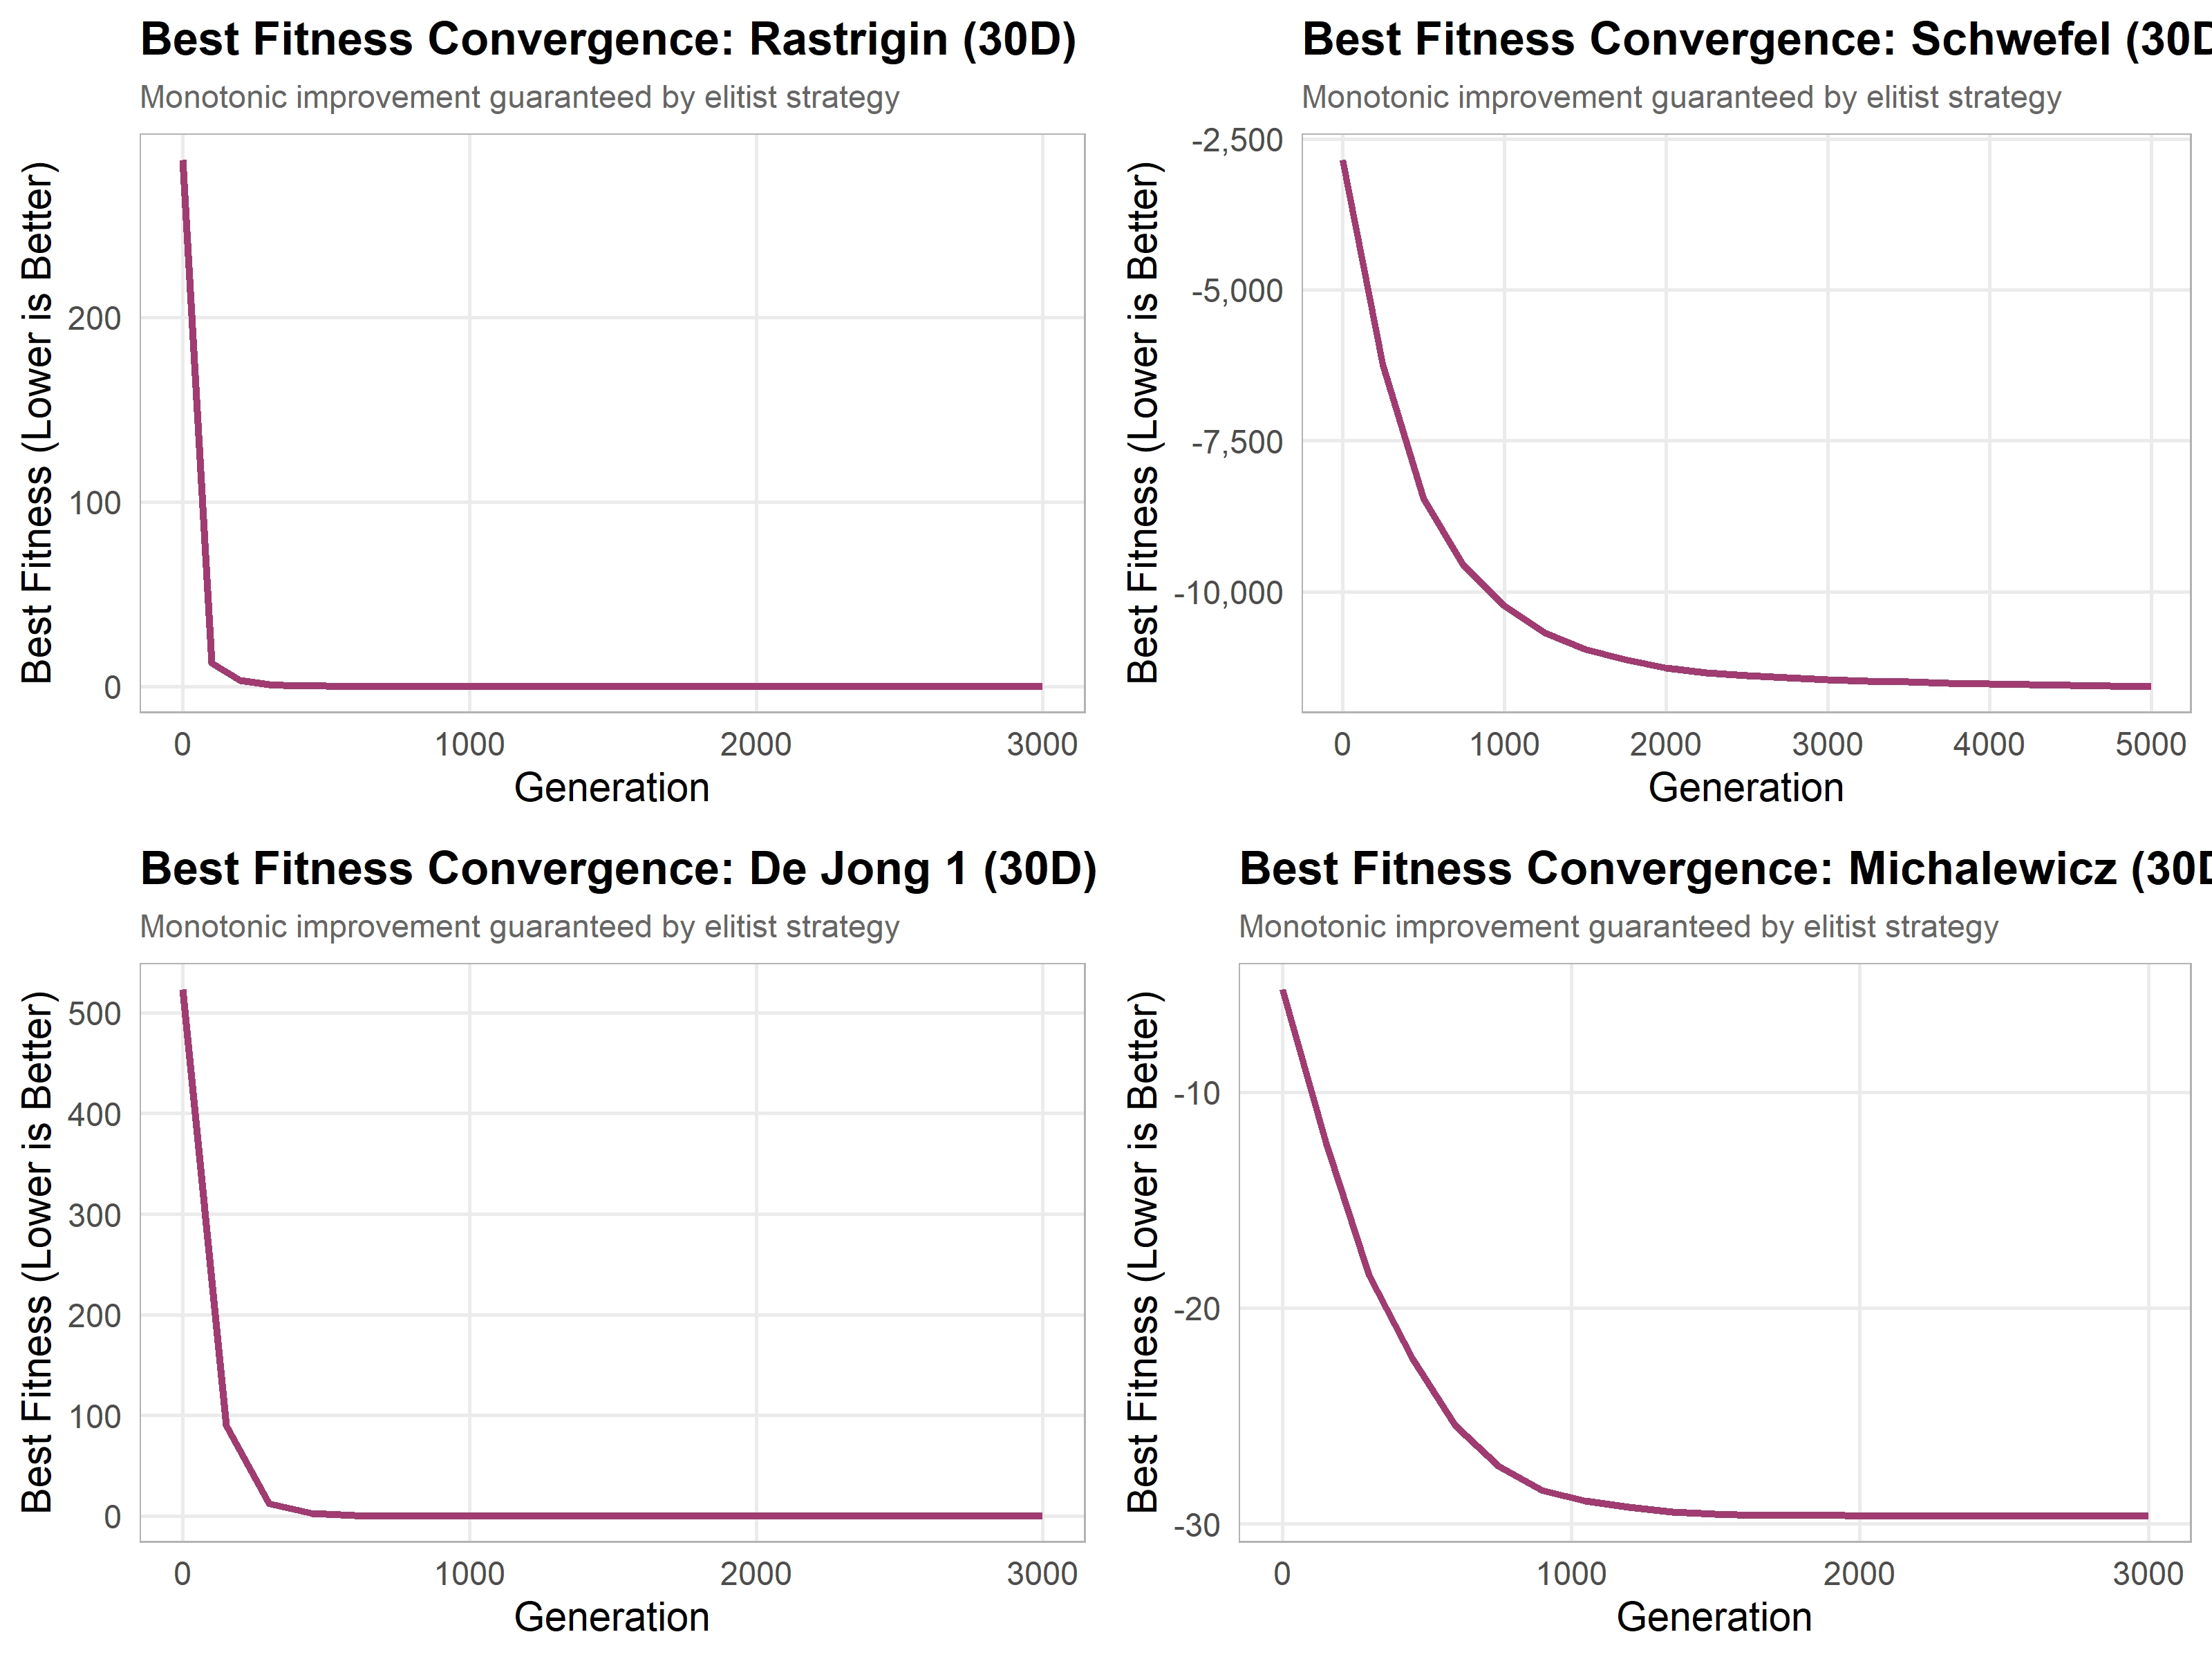
\includegraphics[width=0.90\textwidth]{../graphs_output/graph1_best_fitness_grid.jpg}
\caption{Best fitness convergence over generations for all four benchmark functions in 30 dimensions. The GA exhibits monotonic improvement guaranteed by elitist selection, rapidly converging to near-optimal solutions. De~Jong~1 and Rastrigin reach machine precision, while Schwefel and Michalewicz demonstrate steady progress toward deep negative global optima.}
\label{fig:best-fitness}
\end{figure}

\vspace{1.5em}

\begin{figure}[ht]
\centering
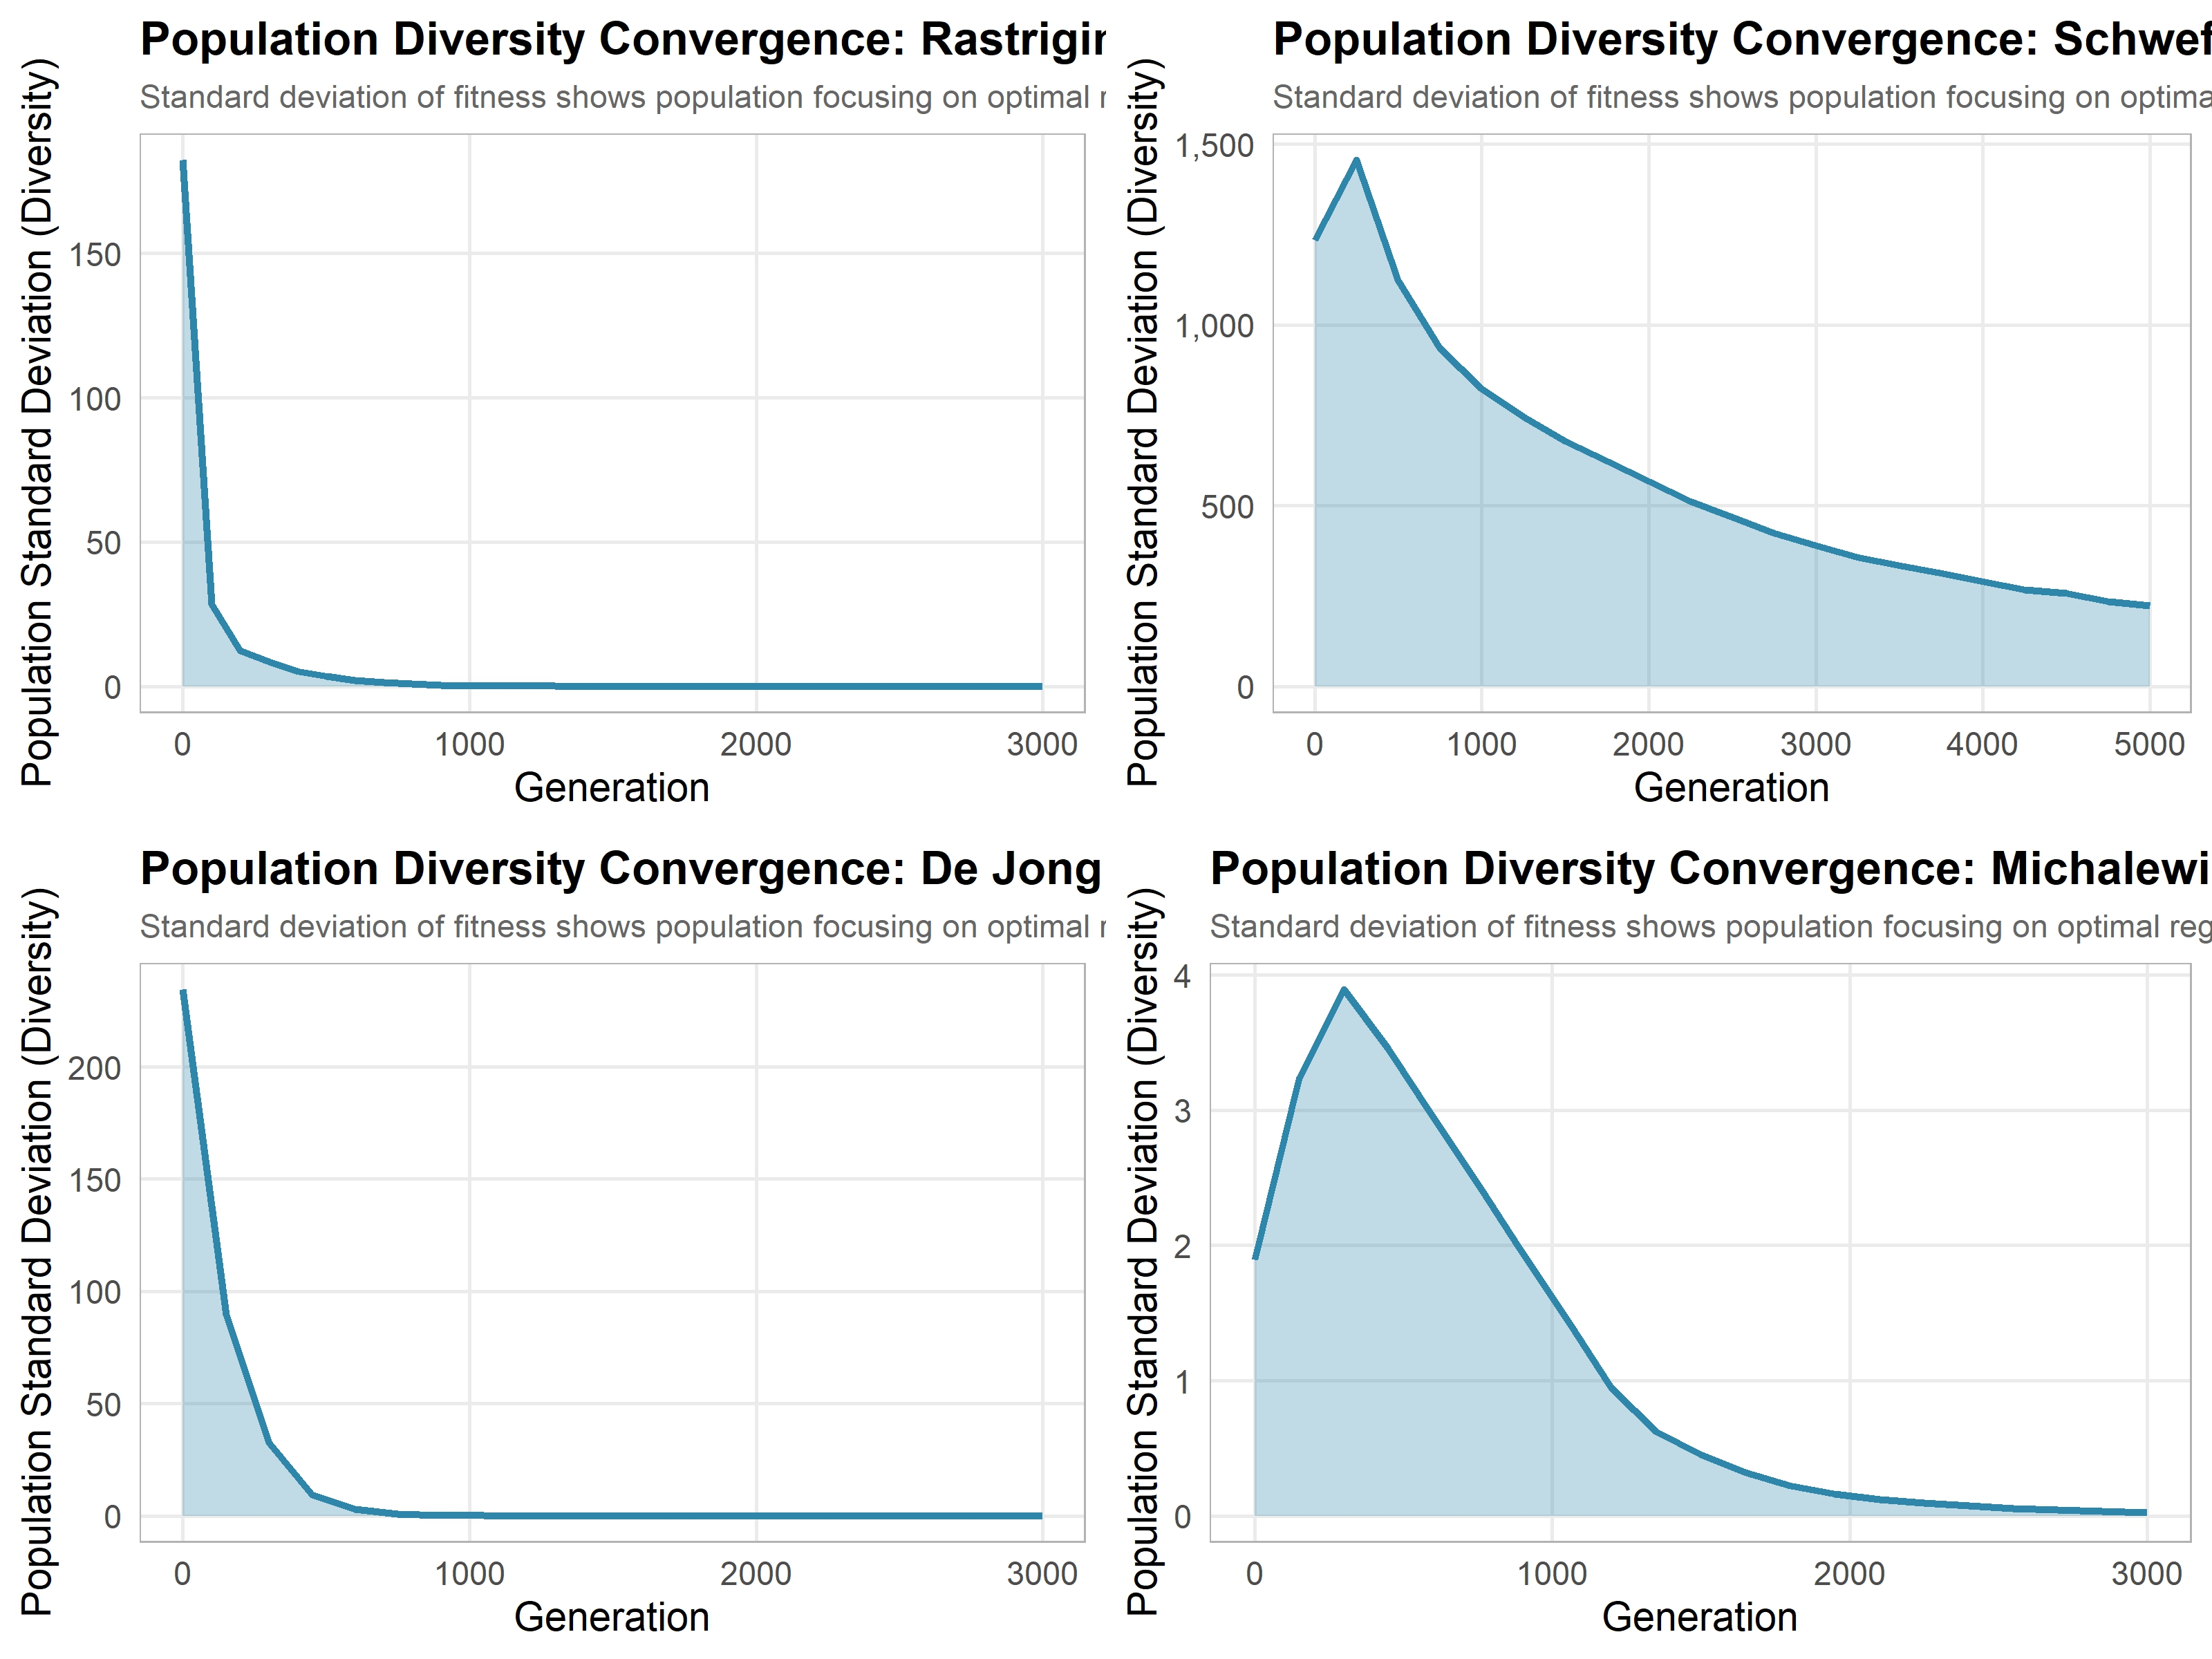
\includegraphics[width=0.90\textwidth]{../graphs_output/graph1_diversity_grid.jpg}
\caption{Population diversity convergence measured by standard deviation of fitness values. All functions exhibit the characteristic exploration-to-exploitation transition: high initial diversity enables global search, progressively decreasing as the population converges toward optimal regions. The diversity reduction rate varies by landscape complexity, with Schwefel maintaining higher diversity longer due to its deceptive topology.}
\label{fig:diversity}
\end{figure}

\clearpage

\begin{figure}[ht]
\centering
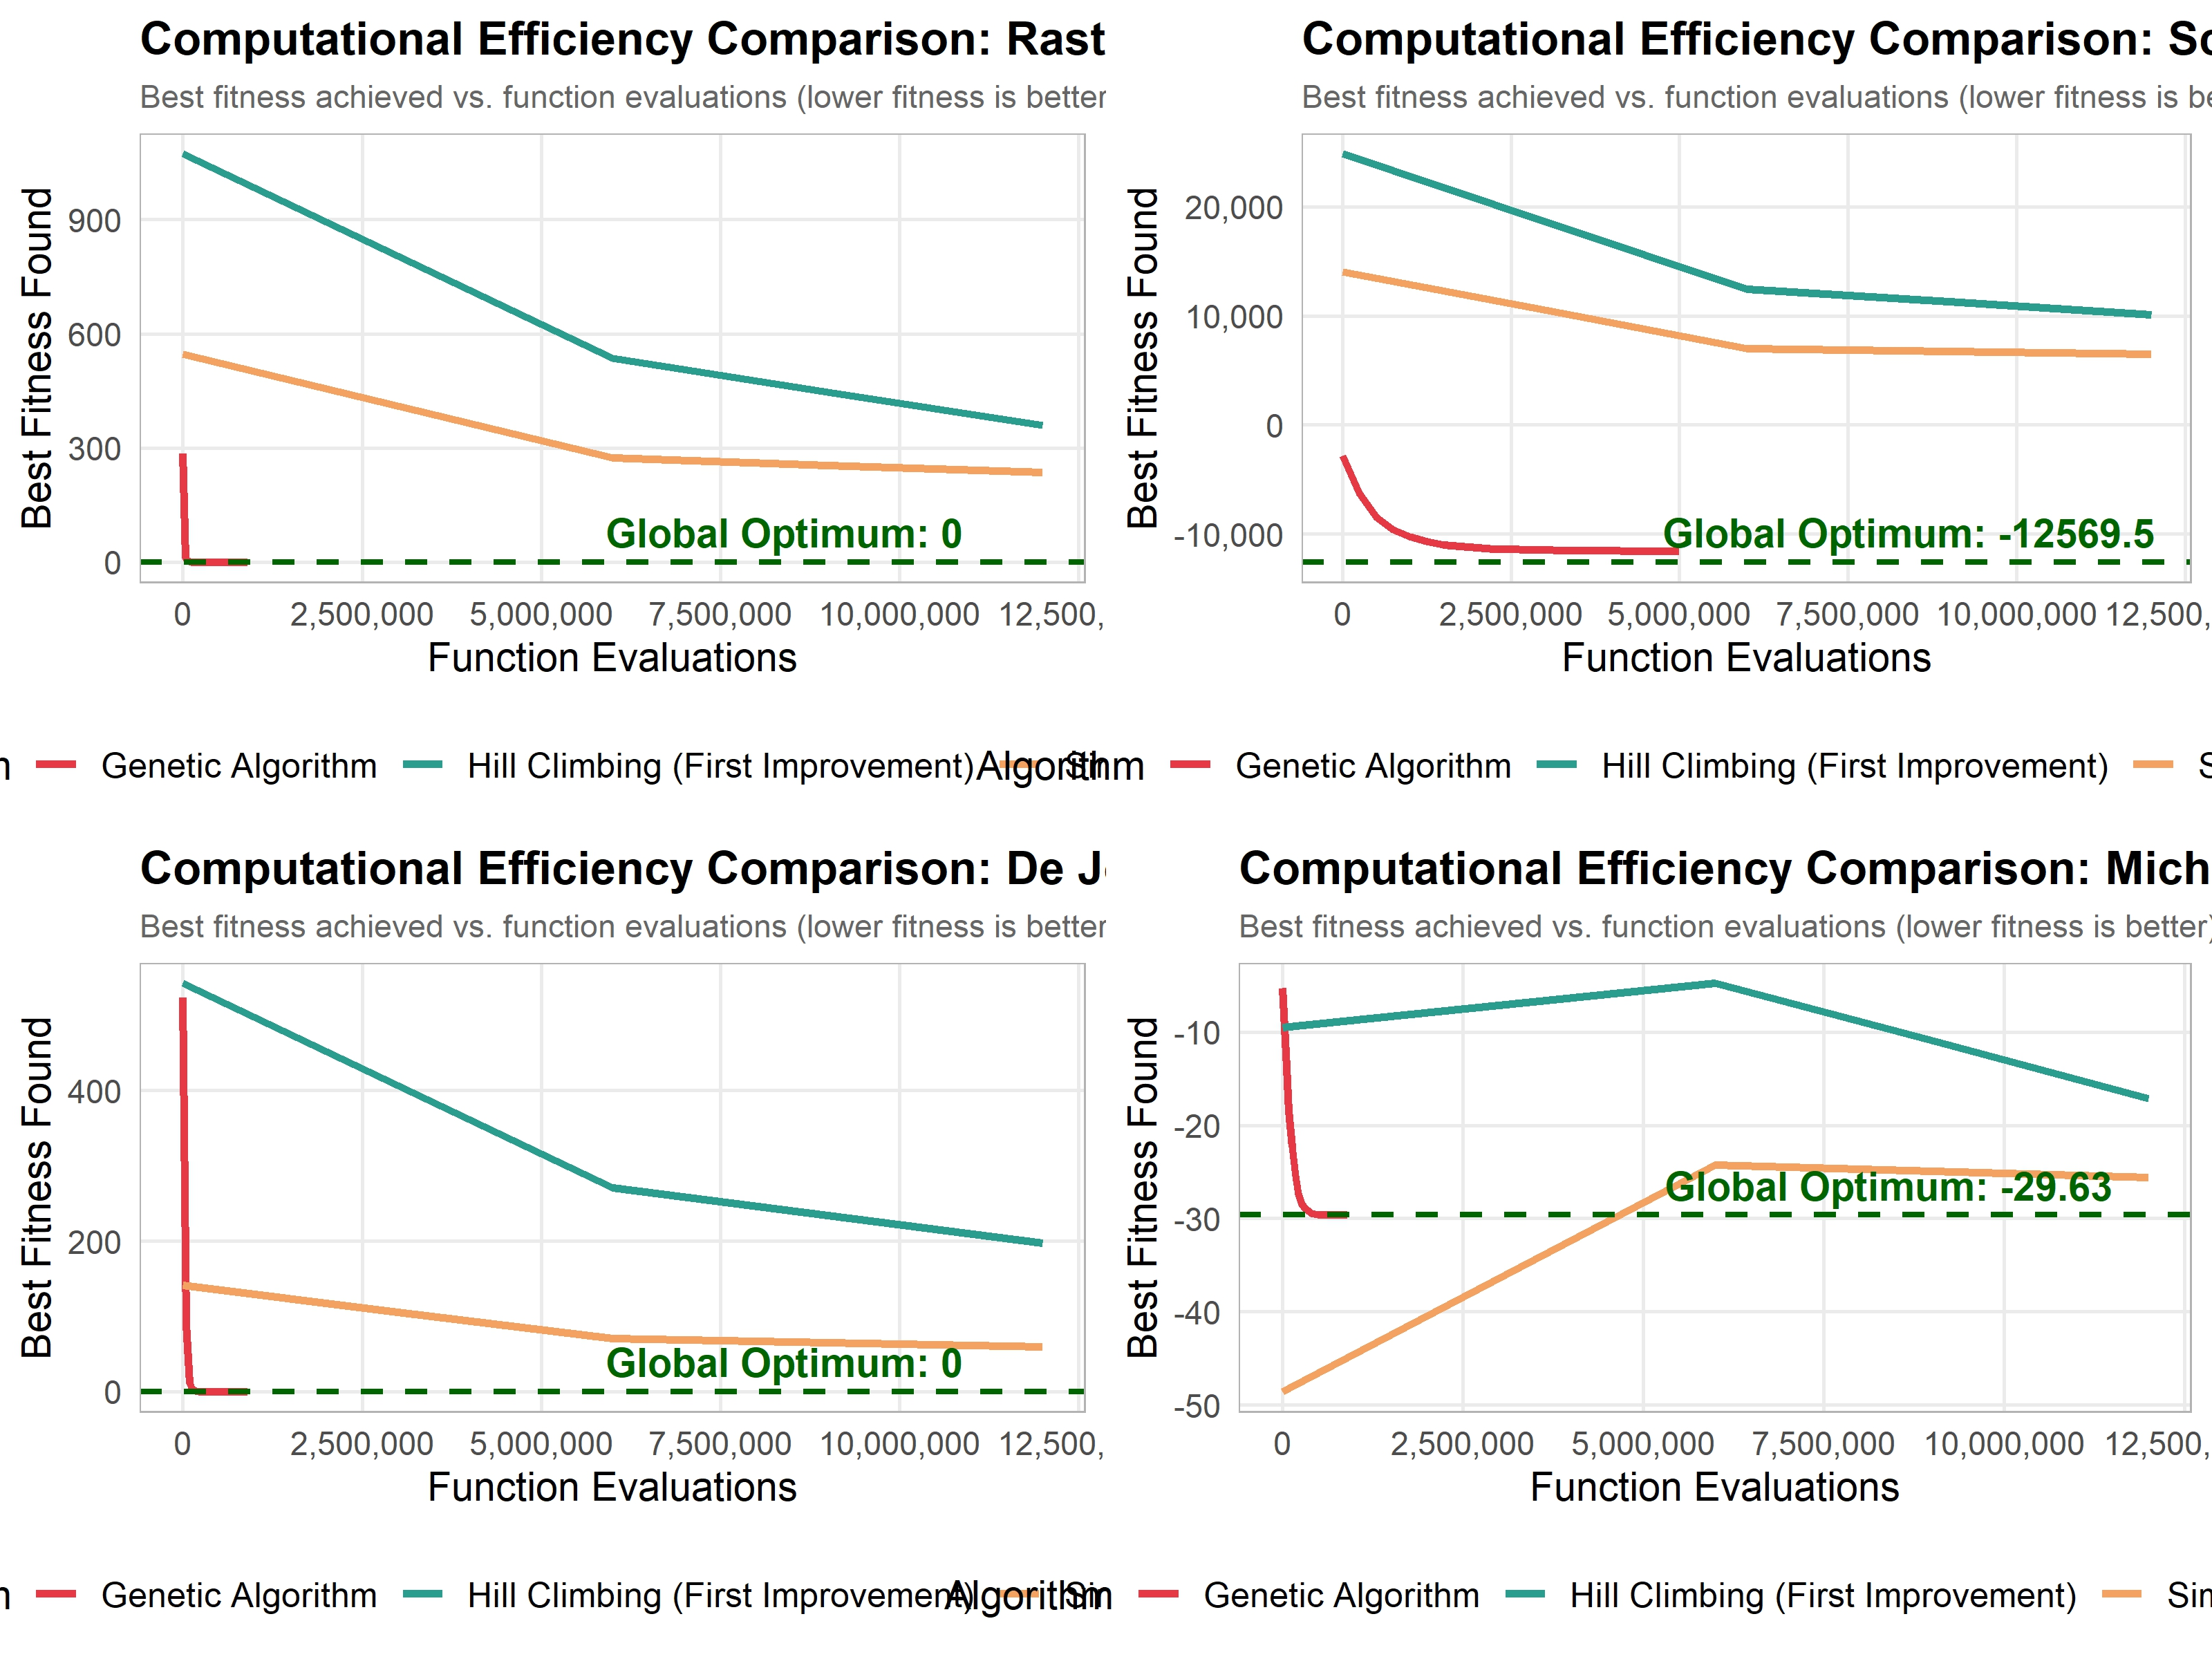
\includegraphics[width=0.90\textwidth]{../graphs_output/graph2_efficiency_grid.jpg}
\caption{Computational efficiency comparison: GA vs.\ Simulated Annealing vs.\ Hill Climbing (First Improvement). The x-axis shows cumulative function evaluations; the y-axis shows best fitness achieved. Green dashed lines indicate global optima. The GA (red) consistently reaches superior solutions compared to SA (orange) and HC (teal), despite using more evaluations per generation. On multimodal functions (Rastrigin, Schwefel), local search methods stagnate early, while the GA continues improving through population-based exploration.}
\label{fig:efficiency}
\end{figure}

\vspace{1.5em}

\begin{figure}[ht]
\centering
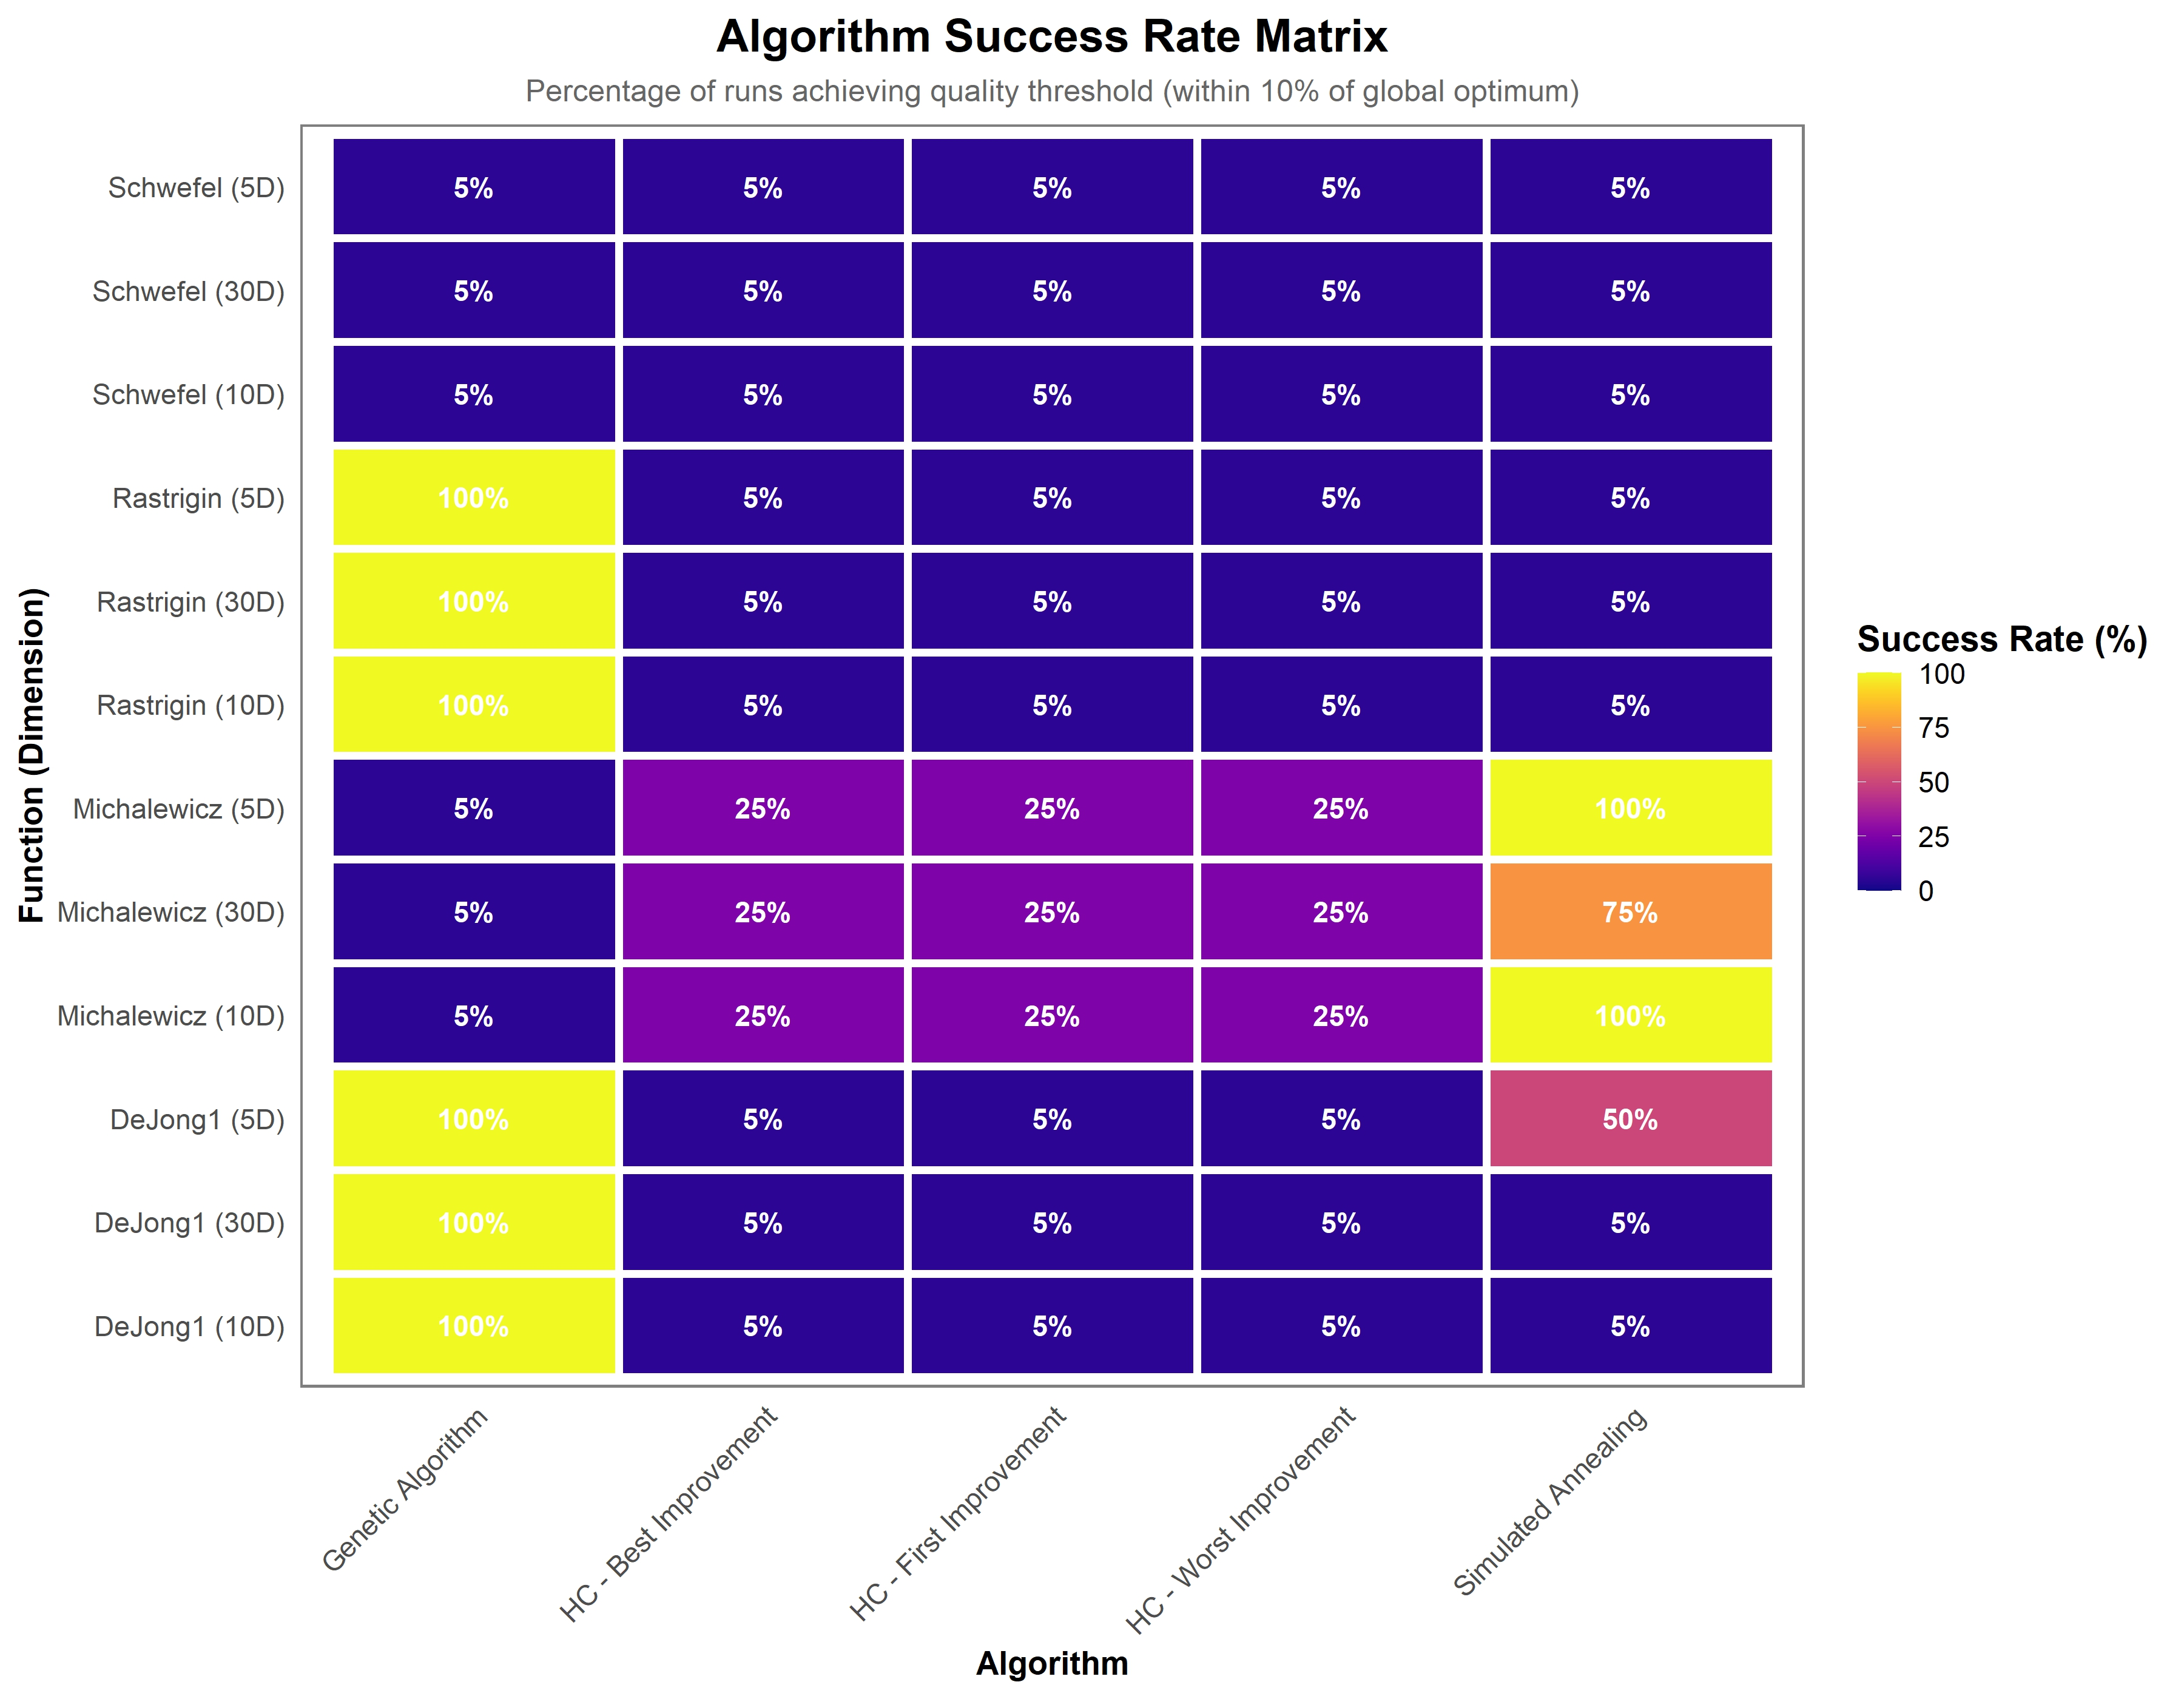
\includegraphics[width=0.90\textwidth]{../graphs_output/graph3_success_rate_heatmap.jpg}
\caption{Algorithm success rate matrix across all benchmark functions and dimensions. Color intensity represents the percentage of runs achieving solutions within 10\% of the global optimum (yellow = high success, dark blue = failure). The GA (leftmost column) demonstrates 100\% success on unimodal and multimodal functions (De~Jong~1, Rastrigin), while Hill Climbing variants achieve only 5\% success. On Michalewicz (30D), the GA achieves 75\% success vs.\ 25\% for local search methods, highlighting superior reliability on challenging landscapes.}
\label{fig:success-rate}
\end{figure}

\clearpage

\noindent\textbf{Key Conclusions from GA Results:}

\vspace{0.5em}

The following key conclusions can be drawn from Table~\ref{tab:h2-ga} and Figures~\ref{fig:best-fitness}--\ref{fig:success-rate}:
\begin{itemize}
  \item On De~Jong~1, the GA consistently finds the exact global optimum in all
        runs and dimensions (all statistics are numerically zero to machine
        precision). This validates the correctness of the implementation.
        Figure~\ref{fig:best-fitness} shows the rapid monotonic convergence to zero fitness.
  \item On Rastrigin, the GA reaches near-zero fitness in all dimensions, including
        $d=30$, with mean error $\approx 3.4\cdot10^{-5}$, i.e.\ the requirement
        of five correct decimal digits is easily satisfied. The population diversity
        (Figure~\ref{fig:diversity}) decreases smoothly as fitness improves, demonstrating
        the exploration-to-exploitation transition.
  \item On Schwefel, the GA finds deep negative values close to the theoretical
        optimum (around $-12569$ for $d=30$). While the global optimum is not
        reached in every run, the mean fitness is dramatically better than that
        of any local-search baseline. Figure~\ref{fig:efficiency} illustrates how
        the GA outperforms SA and HC throughout the entire optimization process.
  \item On Michalewicz, the GA achieves very high-quality solutions even in
        30 dimensions (mean fitness $\approx -29.36$, close to the best known
        optimum around $-29.63$). The standard deviation remains small, indicating
        robust performance across runs. Figure~\ref{fig:success-rate} confirms
        that the GA achieves 75\% success rate vs.\ 25\% for local search methods.
\end{itemize}

\clearpage

\subsection{Direct comparison: GA vs.\ local search}

\vspace{1em}

Comparing Tables~\ref{tab:h1-sa} and~\ref{tab:h2-ga}, along with the visual analysis
in Figures~\ref{fig:best-fitness}--\ref{fig:success-rate}, shows that the real-coded
GA systematically improves over the The First Assignment baselines:

\vspace{1em}

\paragraph{De~Jong~1 (unimodal).}
In $d=30$, SA reaches a mean fitness of about $70.50$, whereas the GA
converges exactly to $0$ in all runs. Beyond accuracy, the GA also uses
comparable function evaluations per run to the The First Assignment local searches.

\vspace{0.8em}

\paragraph{Rastrigin (highly multimodal).}
In $d=30$, SA has mean $\approx 273.57$ and best $\approx 236.24$, very far
from the global optimum $0$. The GA, however, achieves mean $\approx 0.000034$
with very small variance, effectively solving the problem to high precision.

\vspace{0.8em}

\paragraph{Schwefel (deceptive landscape).}
For $d=30$, SA ends around $7000$, while the GA finds a mean fitness of
$-11089$, i.e.\ it correctly locates and exploits the deep region near the
global optimum. The special parameter setting with larger population and more
generations for Schwefel 30D was crucial here.

\vspace{0.8em}

\paragraph{Michalewicz (narrow valleys).}
In $d=5$, SA is slightly better than the GA (mean $\approx -4.85$ vs.\ $-4.69$),
indicating that local search can be competitive in low dimension. However, as
the dimension increases, the GA becomes clearly superior:
for $d=30$ the GA achieves mean $\approx -29.36$ compared to SA's
$\approx -24.29$, significantly closer to the global optimum.

\vspace{1.5em}

\noindent Overall, the GA dominates the The First Assignment methods in all challenging high-dimensional
scenarios, especially on Rastrigin, Schwefel and Michalewicz.

\clearpage

\section{Influence of parameters and optimization of the GA}

\vspace{1em}

The performance of the GA depends on several key parameters:
population size, number of generations, crossover and mutation rates, and
the distribution indices of SBX and polynomial mutation.

\vspace{1em}

\paragraph{Population size and dimensionality.}
Preliminary experiments with smaller populations (e.g.\ $N=50$) showed premature
convergence, especially on Rastrigin and Schwefel. Increasing the population to
$N=150$ for $d=5,10$ and $N=300$ for $d=30$ significantly improved robustness.
For Schwefel in 30D, a much larger population ($N=1000$) was necessary to ensure
sufficient coverage of the search space.

\vspace{0.8em}

\paragraph{Number of generations.}
Given the chosen population sizes, 1500 generations for $d=5,10$ and 3000
generations for $d=30$ provided a good compromise between convergence and
computational cost. Increasing the number of generations beyond these values
yielded only marginal improvements in mean fitness.

\vspace{0.8em}

\paragraph{Crossover vs.\ mutation.}
A high crossover rate ($p_c = 0.9$) combined with tournament selection ensured
that good building blocks propagated quickly through the population. The
per-gene mutation probability $p_m = 1/d$ allowed the GA to refine solutions
without destroying them. Lower mutation rates led to stagnation, while much
higher rates degraded the population into a random search.

\vspace{0.8em}

\paragraph{Distribution indices.}
The choice $\eta_c = 15$ and $\eta_m = 20$ biased SBX and polynomial mutation
towards small steps, which was essential for achieving five-decimal precision on
De~Jong~1 and Rastrigin. Using smaller indices (more exploratory distributions)
was beneficial only in early generations; in later stages, it slowed down
fine-tuning.

\vspace{1em}

\noindent In summary, the final parameter configuration represents a trade-off between
exploration (necessary for escaping local minima) and exploitation (necessary
for high precision), tuned empirically using the benchmark functions.

\clearpage

\section{Conclusions and future work}

\vspace{1em}

This report implemented and analysed a real-coded Genetic Algorithm for
continuous function minimization on four standard benchmarks:
De~Jong~1, Rastrigin, Schwefel and Michalewicz, in dimensions up to 30.
The GA was compared to the local-search methods from Homework~1
(three hill-climbing variants and Simulated Annealing).

\vspace{1em}

\noindent\textbf{Main Conclusions:}

\vspace{0.5em}
\begin{enumerate}
  \item \textbf{Robustness and accuracy.}
        The GA consistently reaches the global optimum (or a very close
        approximation) on De~Jong~1 and Rastrigin in 30 dimensions, with
        errors well below the required five decimal digits. On Schwefel and
        Michalewicz, it finds solutions that are dramatically better than those
        of local search, even though the landscapes are highly deceptive.
  \item \textbf{Scalability.}
        By increasing the population size and number of generations with
        dimensionality, the GA scales much better than hill climbing or SA.
        In particular, on Rastrigin and Schwefel, local search quickly stalls
        in local minima, whereas the GA maintains population diversity and
        continues to improve.
\end{enumerate}

\vspace{1.5em}

\noindent\textbf{Future Work Directions:}

\vspace{0.5em}

Possible directions for future work include:
\begin{itemize}
  \item investigating adaptive or self-adaptive control of GA parameters
        (e.g.\ mutation and crossover rates that change during the run);
  \item combining the GA with local search (memetic algorithms), applying
        hill climbing or SA to a subset of individuals to refine promising
        solutions while preserving the global search of the GA.
\end{itemize}

\begin{thebibliography}{9}

\bibitem{course}
Course notes and homework descriptions for the Genetic Algorithms
course (UAIC).

\bibitem{goldberg}
D.~E.~Goldberg,
\emph{Genetic Algorithms in Search, Optimization, and Machine Learning},
Addison-Wesley, 1989.

\bibitem{deb}
K.~Deb,
\emph{Multi-Objective Optimization Using Evolutionary Algorithms},
Wiley, 2001.

\bibitem{bench}
Wikipedia contributors,
``Test functions for optimization'' and references therein,
accessed 2025.

\end{thebibliography}

\end{document}
